\section{Oscillation} \label{section:oscillation}

\subsection{oscillatory motion}

\begin{ilight}
	\keypoint{oscillation} refers to a repetitive back and forth motion about it \emph{equilibrium position}
\end{ilight}

the equilibrium point is a point where all forces on oscillator are balanced

release an object from its equilibrium position from rest, it will stay at rest

examples of oscillation includes pendulum of a clock, vibrating string, swing, etc.


\subsubsection{amplitude, period, frequency}

to describe motion of an oscillator, we define the following quantities:

\cmt \keypoint{displacement} ($x$): distance from the equilibrium position

\cmt \keypoint{amplitude} ($x_0$)\index{amplitude}: maximum displacement from the equilibrium position

\cmt \keypoint{period} ($T$): time for one complete oscillation

\cmt \keypoint{frequency} ($f$): number of oscillations per unit time

frequency is related to period as: $\boxed{f=\frac{1}{T}}$

\vspace*{\baselineskip}

displacement $x$ varies with time $t$ repetitively, so we can plot an $x$-$t$ graph

amplitude $x_0$ and period $T$ are labelled on the graph


\begin{figure}[ht]
\begin{center}
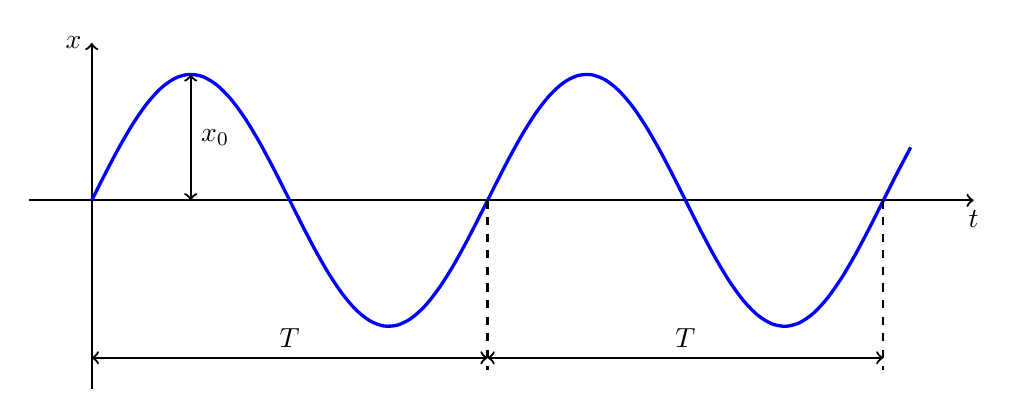
\begin{tikzpicture}[xscale=0.8,yscale=0.8]
\draw [thick, ->] (-1,0) --(14,0) node[below]{$t$};
\draw [thick, ->] (0,-3) --(0,2.5) node[left]{$x$};
\draw [very thick,color=blue,domain=0:13,smooth,samples=60,variable=\x] plot (\x,{2*sin(\x r)});
\draw [thick,<->] (0,-2.5) -- (2*pi,-2.5)  node[above,midway]{$T$};
\draw [thick,<->] (2*pi,-2.5) -- (4*pi,-2.5)  node[above,midway]{$T$};
\draw [thick,dashed] (2*pi,0) -- (2*pi,-2.7) (4*pi,0) -- (4*pi,-2.7);
\draw [thick,<->] (pi/2,0) --  (pi/2,2) node[right,midway]{$x_0$};
\end{tikzpicture}

displacement-time graph for a typical oscillator
\end{center}
\end{figure}


\subsubsection{phase angle}
the point that an oscillator has reached within a complete cycle is called \keypoint{phase angle}\index{phase angle} ($\phi$)

\cmt unit of phase angle: $[\phi] = \text{rad}$

it looks like an angle, but better think of it as a number telling fraction of a complete cycle

\cmt we use \keypoint{phase difference} $\Delta\phi$ to compare how much one oscillator is ahead of another

$\Delta\phi$ is found in terms of fraction of an oscillation: $\Delta\phi = \frac{\Delta t}{T} \times 2\pi $ (also measured in radians)



%\begin{center}
%\begin{minipage}{0.48\textwidth}
%
%\example{$\frac{1}{4}T \, \longleftrightarrow \, \Delta\phi = \frac{1}{4}\times 2\pi = \frac{1}{2}\pi$}
%\begin{center}
%\begin{tikzpicture}[xscale=0.7,yscale=0.6]
%\draw [thick, ->] (-1,0) --(8,0) node[below]{$t$};
%\draw [thick, ->] (0,-3) --(0,2.5) node[left]{$x$};
%\draw [thick,color=blue,domain=0:7,smooth,variable=\x] plot (\x,{2*sin(\x r)});
%\draw [thick,dashed,color=blue,domain=0:7,smooth,variable=\x] plot (\x,{2*sin(((\x - pi/2) r)});
%\end{tikzpicture}
%\end{center}
%
%\end{minipage}
%\begin{minipage}{0.48\textwidth}
%\example{$\frac{1}{2}T \, \longleftrightarrow \, \Delta\phi = \frac{1}{2}\times 2\pi = \pi$}
%\begin{center}
%\begin{tikzpicture}[xscale=0.7,yscale=0.6]
%\draw [thick, ->] (-1,0) --(8,0) node[below]{$t$};
%\draw [thick, ->] (0,-3) --(0,2.5) node[left]{$x$};
%\draw [thick,color=blue,domain=0:7,smooth,variable=\x] plot (\x,{2*sin(\x r)});
%\draw [thick,dashed,color=blue,domain=0:7,smooth,variable=\x] plot (\x,{2*sin(((\x - pi) r)});
%\end{tikzpicture}
%\end{center}
%\end{minipage}
%\end{center}

\example{Compare the two oscillations from the $x$-$t$ graph below.}

\begin{wrapfigure}{l}{6cm}
	\vspace*{-12pt}
		\centering
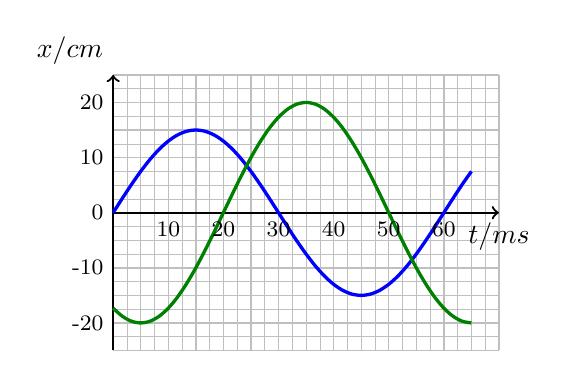
\begin{tikzpicture}[scale=0.7]
\draw[style=help lines,step=0.25,gray!50] (0,-2.5) grid (7,2.5);
\draw[step=0.5,gray!50] (0,-2.5) grid (7,2.5);
\draw [thick, ->] (0,0) --(7,0) node[below]{$t/\text{ms}$};
\draw [thick, ->] (0,-2.5) --(0,2.5) node[above left]{$x/\text{cm}$};
\draw [very thick,color=blue,domain=0:6.5,samples=40,smooth,variable=\x] plot (\x,{1.5*sin((\x*pi/3) r)});
\draw [very thick,color=Green,domain=0:6.5,samples=40,smooth,variable=\x] plot (\x,{2*sin(((\x- 2)*pi/3 ) r)});
\foreach \s in {10,20,...,60}
  \draw (\s/10,0) node[below]{\footnotesize{\s}};
\foreach \s in {-20,-10,...,20}
    \draw (0,\s/10) node[left]{\footnotesize{\s}};
\end{tikzpicture}
\vspace*{-25pt}
\end{wrapfigure}

\sol both have period $T=60$ ms

frequency $f=\frac{1}{60\times10^{-3}} \approx 16.7$ Hz

they are of different amplitudes

one has $x_0=15$ cm, the other has $x_0=20$ cm

time difference: $\Delta t = 20$ ms

phase difference: $\Delta \phi = \frac{\Delta t}{T} \times 2\pi = \frac{20}{60} \times 2\pi = \frac{2\pi}{3} \text{ rad}$



\subsubsection{acceleration \& restoring force}
for any oscillatory motion, consider its velocity and acceleration at various positions

its acceleration must be always pointing towards the equilibrium position

resultant force always acts in the direction to restore the system back to its equilibrium point, this net force is known as the \keypoint{restoring force}\index{restoring force}

if at equilibrium position, then no acceleration or restoring force





\subsection{simple harmonic oscillation}

\begin{ilight}
	if an oscillator has an acceleration always proportional to its displacement from the equilibrium position, and acceleration is in opposite direction to displacement, then the oscillator is performing \keypoint{simple harmonic motion}\index{simple harmonic motion}
\end{ilight}

many phenomena can be approximated by simple harmonics

examples are motion of a pendulum, molecular vibrations, etc.

complicated motions can be decomposed into a set of simple harmonics

simple harmonic motion provides a basis for the study of many complicated motions
\footnote{This can be done through a mathematical technique known as \emph{Fourier analysis}. For example, a uniform circular motion can be considered as the combination of two simple harmonic motion in $x$- and $y$-directions.}

\subsubsection{equation of motion}

defining equation for simple harmonics can be written as $\boxed{a=-\omega^2 x}$

$\omega$ is some constant, so $a$ is proportional to $x$

the minus sign shows $a$ and $x$ are in opposite directions

\vspace*{\baselineskip} 

general solution to this this equation of motion\footnote{You probably know that acceleration can be written as the second derivative of displacement: $a=\frac{\dd^2 x}{\dd t^2}$, so $a=-\omega^2 x$ is equivalent to $\frac{\dd^2 x}{\dd t^2} + \omega^2 x = 0$, which a \emph{second-order differential equation}. If you do not know how to solve it, you may have the chance to study this in an advanced calculus course.} takes the form: $\boxed{x=x_0\sin(\omega t+\phi)}$

$x_0$ represents the amplitude, $\omega$ is called the angular frequency, $\phi$ is the phase angle

\subsubsection*{angular frequency}

\cmt \keypoint{angular frequency}\index{angular frequency}  satisfies the relation: $\boxed{\omega=\frac{2\pi}{T}=2\pi f}$

\cmt unit of angular frequency: $[\omega] = \rad\cdot\text{s}^{-1}$

\cmt angular frequency $\omega$ is determined by the system's \emph{physical constants} only

if an object is set to oscillate \emph{freely} with no external force, its period will always be the same

frequency of an free oscillatory system is called the \keypoint{natural frequency}

\subsubsection*{phase angle}


\cmt phase angle $\phi$ is dependent on \emph{initial conditions} (e.g. initial position and initial speed at $t=0$?)

\cmt in many cases, phase angle term can be avoided if a suitable trigonometric function is chosen



\example{A simple harmonic oscillator is displaced by 6.0 cm from its rest position and let go at $t=0$. Given that the period of this system is 0.80 s, state an equation for its displacement-time relation.}

\begin{wrapfigure}{r}{4.8cm}
	\centering
	\vspace*{-30pt}
	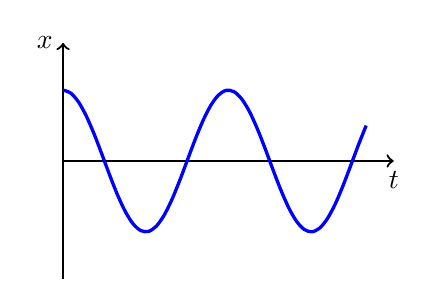
\begin{tikzpicture}[xscale=0.7,yscale=0.6]
	\draw [thick, ->] (0,0) --(6,0) node[below]{$t$};
	\draw [thick, ->] (0,-2.5) --(0,2.5) node[left]{$x$};
	\draw [very thick,color=blue,domain=0:5.5,samples=40,smooth,variable=\x] plot (\x,{1.5*cos((\x*pi/1.5) r)});
	\end{tikzpicture}
	\vspace*{-5pt}
\end{wrapfigure}

\sol angular frequency: $\omega = \frac{2\pi}{T} = \frac{2\pi}{0.80} = \frac{5\pi}{2}\pi \radps$

initial displacement $x(0) = +x_0 = 6.0 \text{ cm}$

for displacement-time relation, we use cosine function 
\begin{equation*}
x(t) = x_0 \cos\omega t \RA x = 6.0\cos\left(\frac{5\pi}{2} t\right) \teoe
\end{equation*}


\example{A simple harmonic oscillator is initially at rest. At $t=0$, it is given an initial speed in the negative direction. Given that the frequency is 1.5 Hz and the amplitude is 5.0 cm, state an equation for its displacement-time relation.}

\begin{wrapfigure}{r}{4.8cm}
	\centering
	\vspace*{-30pt}
	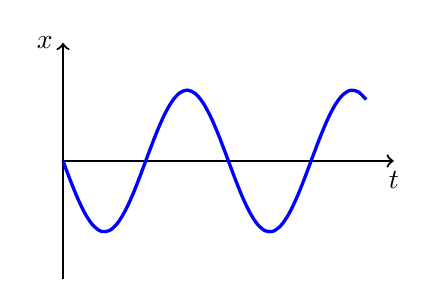
\begin{tikzpicture}[xscale=0.7,yscale=0.6]
	\draw [thick, ->] (0,0) --(6,0) node[below]{$t$};
	\draw [thick, ->] (0,-2.5) --(0,2.5) node[left]{$x$};
	\draw [very thick,color=blue,domain=0:5.5,samples=40,smooth,variable=\x] plot (\x,{-1.5*sin((\x*pi/1.5) r)});
	\end{tikzpicture}
\end{wrapfigure}

\sol angular frequency: $\omega = 2\pi f = 2\pi\times1.5 = 3 \pi \radps$

initial displacement $x(0) = 0$

for displacement-time relation, we use sine function 
\begin{equation*}
x(t) = - x_0 \cos\omega t \RA x = - 5.0\sin(3\pi t) \teoe
\end{equation*}
	
\subsubsection{examples of simple harmonics}

\subsubsection*{mass-spring oscillator}

a mass-spring oscillator system consists of a block of mass $m$ and an ideal spring

\begin{figure}[ht]
	\centering
		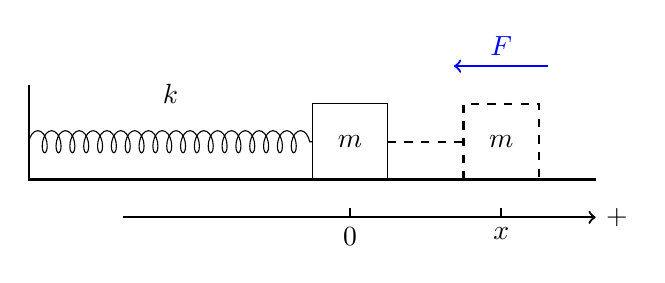
\begin{tikzpicture}[scale=1.2]
		\draw (0,0) rectangle (.8,.8);
		\draw[dashed,thick] (1.6,0) rectangle (2.4,.8);
		\draw[dashed,thick] (.8,.4) -- (1.6,.4);
		\draw (0.4,0.4) node{$m$};
		\draw (2,0.4) node{$m$};
		\draw (-1.5,0.7) node[above]{$k$};
		\draw [thick] (3,0) -- (-3,0) -- (-3, 1);
		\draw[decorate, decoration={coil,amplitude=4pt, segment length=5pt}] (-3,0.4) -- (0,0.4);
		\draw [thick,->,blue] (2.5,1.2) -- (1.5,1.2) node[midway,above]{$F$};
		\draw [thick,->] (-2,-0.4) -- (0.4,-0.4) node[below]{$0$} -- (3,-0.4) node[right]{$+$};
		\draw [thick ] (0.4,-0.4) -- (0.4,-0.3);
		\draw [thick ] (2,-0.4) node[below]{$x$} -- (2,-0.3);
		\end{tikzpicture}
		
		\vspace*{5pt}
		
		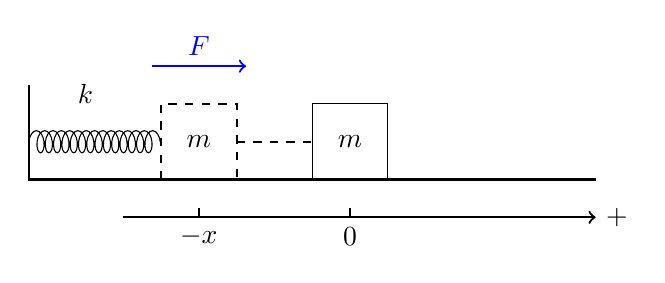
\begin{tikzpicture}[scale=1.2]
		\draw (0,0) rectangle (.8,.8);
		\draw[dashed,thick] (-1.6,0) rectangle (-0.8,.8);
		\draw[dashed,thick] (-0.8,.4) -- (0,.4);
		\draw (0.4,0.4) node{$m$};
		\draw (-1.2,0.4) node{$m$};
		\draw (-2.4,0.7) node[above]{$k$};
		\draw [thick] (3,0) -- (-3,0) -- (-3, 1);
		\draw[decorate, decoration={coil,amplitude=4pt, segment length=3pt}] (-3,0.4) -- (-1.6,0.4);
		\draw [thick,->,blue] (-1.7,1.2) -- (-0.7,1.2) node[midway,above]{$F$};
		\draw [thick,->] (-2,-0.4) -- (0.4,-0.4) node[below]{$0$} -- (3,-0.4) node[right]{$+$};
		\draw [thick] (0.4,-0.4) -- (0.4,-0.3);
		\draw [thick ] (-1.2,-0.4) node[below]{$-x$} -- (-1.2,-0.3);
		\end{tikzpicture}
		
	restoring force acting on the ideal mass-spring oscillator
\end{figure}

when a spring is stretched or compressed by a mass, the spring develops a restoring force

magnitude of this force obeys \emph{Hooke's law}: $F=kx$ 

direction of this force is in opposite direction to displacement $x$

take vector nature of force into account, we find
\begin{equation*}
	\fnet = ma \RA -kx = ma \RA a=-\frac{k}{m}x
\end{equation*}

spring constant $k$ and mass $m$ are constants, so $a \propto x$

negative sign shows $a$ and $x$ are in opposite directions

so mass-spring oscillator executes simple harmonic motion

\vspace*{\baselineskip}

compare with $a=-\omega^2x \RA \omega^2 = \frac{k}{m} \RA \boxed{\omega = \sqrt{\frac{k}{m}}}$

period of mass-spring oscillator: $T=\frac{2\pi}{\omega} \RA T =2\pi\sqrt{\frac{m}{k}}$

\cmt period and frequency are solely determined by mass of oscillator $m$ and spring constant $k$

identical mass-spring systems will oscillate at same frequency no matter what amplitude

\cmt $m \up \ra T \up$, greater mass means greater inertia, oscillation becomes slower

\cmt $k \up \ra T \down$, greater $k$ means stiffer spring, greater restoring force makes oscillation go faster



\subsubsection*{simple pendulum}

a simple pendulum is set up by hanging a bob on a light cord from a fixed point

displace the bob by some angle and release from rest, it can swing freely

\begin{wrapfigure}{l}{4.8cm}
	\centering
		\begin{tikzpicture}[scale=1]
			\draw[dashed] (0,0) -- (0,-6.4) node[below]{$0$};
			\draw (0,-1) arc(-90:-75:1);
			\draw[orange,<->] (-81:4) arc(-81:-99:4);
			\draw (-80:1) node[below]{$\theta$};
			\draw[thick,blue,->] (-75:4) -- ++ (0,-1.932) node[right]{$mg$};
			\draw[thick,blue,->] (-75:4) -- ++ (105:2) node[above  right]{$T$};
			\draw[thick, fill] (0,0) -- (-75:4) circle(0.2);
			\draw[thick,->] (-2,-6.4) -- (0,-6.4) -- (2,-6.4) node[right]{$+$};
			\draw [dashed] (1.035,-5.8) -- (1.035,-6.4) node[below]{$x$};
		\end{tikzpicture}
\end{wrapfigure}

one can show this performs simple harmonic motion for \emph{small-angle} oscillation
		
if angular displacement $\theta$ is small, then the pendulum has almost no vertical displacement, the motion can be considered to be purely horizontal
		
vertically: $T\cos\theta \approx mg \quad \xLongrightarrow{\cos\theta\approx1 \text{ as } \theta\to0} \quad T\approx mg$
		
horizontally: $-T\sin\theta = ma \quad \xLongrightarrow{\sin\theta=x/L} \quad a \approx -\frac{g}{L}x$

this shows simple pendulum undergoes simple harmonics
	
compare with defining equation for simple harmonics:

{

\centering

$a=-\omega^2x \RA \omega = \sqrt{\frac{g}{L}}$

}
	
period for a simple pendulum: $\boxed{T= 2\pi\sqrt{\frac{L}{g}}}$

\cmt period and frequency of a pendulum are determined by length of the string $L$ only

as long as angular displacement remains small, frequency does not depend on amplitude

fix length $L$, then simple pendulum oscillates at same frequency no matter what amplitude

\cmt $L \up \ra T \up$, longer pendulums oscillate more slowly

\cmt $g \down \ra T \up$, if there is no gravity ($g=0$), then the bob will not move at all  ($T\to \infty$)

\question{A cylindrical tube of total mass $m$ and cross sectional area $A$ floats upright in a liquid of density $\rho$. When the tube is given a small vertical displacement and released, the magnitude of the resultant force acting on the tube is related to its vertical displacement $y$ by the expression: $\fnet = \rho g A y$. (a) Show that the tube executes simple harmonic motion. (b) Find an expression for the frequency of the oscillation.}

\question{A small glider moves along a horizontal air track and bounces off the buffers at the ends of the track. Assume the track is frictionless and the buffers are perfectly elastic, state and explain whether the glider describes simple harmonic motion.}



\subsubsection{velocity \& acceleration}

displacement of simple harmonic oscillator varies with time as: $x=x_0\sin(\omega t + \phi)$

from this displacement-time relation, we can find velocity and acceleration relations

\subsubsection*{velocity}

to find velocity-time relation, let's recall that velocity $v$ is rate of change of displacement $x$
\begin{equation*}
	v = \frac{\dd x}{\dd t} = \frac{\dd}{\dd t} x_0\sin(\omega t+\phi) \RA \boxed{v(t) = \omega x_0 \cos(\omega t+\phi)}
\end{equation*}

by taking $v^2 + \omega^2 x^2$, the sine and cosine terms can be eliminated, we find:
\begin{equation*}
	v^2 + \omega^2 x^2 = \omega^2 x_0^2 \cos^2(\cdots) + \omega^2 x_0^2 \sin^2(\cdots) = \omega^2 x_0^2
\end{equation*}

this gives velocity-displacement relation: $\boxed{v(x)=\pm \omega\sqrt{x_0^2 - x^2}}$

\cmt at equilibrium position $x=0$, speed is maximum: $\boxed{v_\tmax = \omega x_0}$ 

\cmt when $x=\pm x_0$, oscillator is momentarily at rest: $v=0$ 

\subsubsection*{acceleration}

acceleration-time relation is found by further taking rate of change of velocity $v$
\begin{equation*}
a = \frac{\dd v}{\dd t} = \frac{\dd}{\dd t} \omega x_0 \cos(\omega t+\phi) \RA \boxed{a(t) = - \omega^2 x_0 \sin(\omega t+\phi)}
\end{equation*}

this is actually unnecessary, if we compare this with $x(t)=x_0 \sin(\omega t+\phi)$, we have: $a=-\omega^2 x$

we have recovered the definition for simple harmonics

(if $a \propto x$ and in opposite directions to $x$, then simple harmonic motion)

so acceleration-displacement relation is given by the defining equation explicitly $\boxed{a(x) = -\omega^2 x} $

\cmt at equilibrium position $x=0$, zero acceleration

\cmt when $x=\pm x_0$, acceleration is greatest: $\boxed{a_\tmax = \omega^2 x_0}$ 

\vspace*{\baselineskip}

let's take $x=x_0\sin\omega t$ as example, changes of $x$, $v$, $a$ over time are listed below

\begin{center}
\begin{tabular}{|c|c|c|c|c|c|}
\hline
time $t$ & 0 & $\textstyle{\frac{1}{4}T}$ & $\textstyle{\frac{1}{2}T}$  & $\textstyle{\frac{3}{4}T}$ & $T$ \\ \hline
displacement: $x=x_0\sin\omega t$ & 0 & $+$max & 0 & $-$max & 0 \\ \hline
velocity: $v=\omega x_0\cos \omega t$ & $+$max & 0 & $-$max & 0 & +max \\ \hline
acceleration: $a=-\omega^2x = -\omega^2 x_0\sin\omega t$ & 0 & $-$max & 0 & $+$max & 0 \\
\hline
\end{tabular}
\end{center}

\begin{figure}[ht]
\begin{minipage}{0.48\textwidth}
	\centering
	\begin{tikzpicture}[scale=0.6]
	\draw [thick, ->] (-5,0) --(5.5,0) node[below]{$x$};
	\draw [thick, ->] (0,-4) --(0,4) node[left]{$v$};
	\draw [very thick, blue] (0,0) ellipse (4 and 3);
	\node[below right] at (4,0) {$+x_0$};
	\node[below left] at (-4,0) {$-x_0$};
	\node[above left] at (0,3) {$+v_\tmax$};
	\node[below left] at (0,-3) {$-v_\tmax$};
	\end{tikzpicture}
	
	velocity-displacement graph
\end{minipage}\hfil
\begin{minipage}{0.45\textwidth}
	\centering
	\begin{tikzpicture}[scale=0.6]
	\draw [thick, ->] (-5,0) --(5.5,0) node[below]{$x$};
	\draw [thick, ->] (0,-4) --(0,4) node[left]{$a$};
	\draw [very thick, blue] (4,-3) -- (-4,3);
	\node[above] at (4,0) {$+x_0$};
	\node[below] at (-4,0) {$-x_0$};
	\node[right] at (0,3) {$+a_\tmax$};
	\node[left] at (0,-3) {$-a_\tmax$};
	\draw[dashed] (4,0) -- (4,-3) -- (0,-3);
	\draw[dashed] (-4,0) -- (-4,3) -- (0,3);
	\end{tikzpicture}
	
	acceleration-displacement graph
\end{minipage}

\end{figure}


\example{The motion of a simple pendulum is approximately simple harmonic. As the pendulum swings from one side to the other end, it moves through a distance of $6.0 \text{ cm}$ and the time taken is $1.0 \text{ s}$. (a) State the period and amplitude. (b) Find the greatest speed during the oscillation. (c) Find its speed when displacement $x=1.2\text{ cm}$.}

\sol period: $T=2\times 1.0 = 2.0 \text{ s}$, and amplitude: $x_0 = \frac{1}{2}\times6.0 = 3.0 \text{ cm}$

angular frequency: $\omega = \frac{2\pi}{T} = \frac{2\pi}{2.0} = \pi \radps$

greatest speed: $v_\tmax = \omega x_0 = \pi \times 3.0 \approx 9.4 \text{ cm s}^{-1}$

speed at $1.2 \text{ cm}$: $v = \omega\sqrt{x_0^2 - x^2} = \pi \times \sqrt{3.0^2-1.2^2} \approx 8.6 \text{ cm s}^{-1}$ \eoe



\example{Given the $x$-$t$ graph of a simple harmonic oscillator. (a) Find its speed at $t=0$. (b) Find its greatest speed. (b) Find its acceleration at $t=1.0$ s.}

\begin{wrapfigure}{l}{0.40\linewidth}
\vspace*{-12pt}
\centering
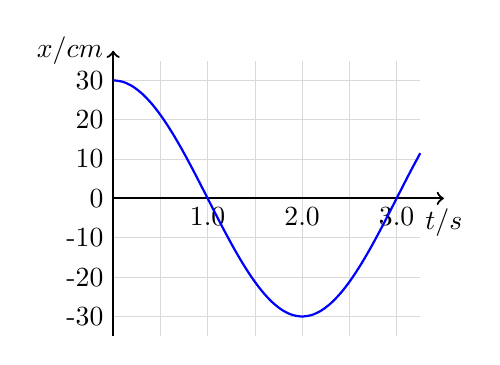
\begin{tikzpicture}[xscale=0.6,yscale=0.5]
\draw[help lines,gray!30] (0,-3.5) grid (6.5,3.5);
\draw [thick, ->] (0,0) --(7,0) node[below]{$t/\text{s}$};
\draw [thick, ->] (0,-3.5) --(0,3.75) node[left]{$x/\text{cm}$};
\foreach \s in {1.0,2.0,3.0}
  \draw (\s*2,0) node[below]{\s};
\foreach \s in {-30,-20,...,30}
    \draw (0,\s/10) node[left]{\s};
\draw [thick,color=blue,domain=0:6.5,samples=32,smooth,variable=\x] plot (\x,{3*cos((\x*pi/4) r)});
\end{tikzpicture}

\end{wrapfigure}


\sol at $t=0$, $x=+x_0 \RA v=0\,$ (zero gradient)

from graph: amplitude $x_0 = 30 \text{ cm}$, period $T=4.0 \text{ s}$

angular frequency: $\omega = \frac{2\pi}{T} = \frac{2\pi}{4} = \frac{\pi}{2} \radps$ 

greatest speed: $v_\tmax = \omega A =  \frac{\pi}{2} \times 30  \approx 47 \cmps$ 

at $t=1.0$ s, $x=0 \RA a=0$

 (equilibrium position so no acceleration) \eoe

\question{Assume the motion of a car engine piston is simple harmonic. The piston completes 3000 oscillations per minute. The amplitude of the oscillation is 4.0 cm. (a) Find the greatest speed. (b) Find the greatest acceleration.}


\subsubsection{vibrational energy}

consider the \emph{ideal} mass-spring oscillator, its vibrational energy consists of two parts:

\begin{compactitem}
	\item[-] kinetic energy of the mass: $E_k = \frac{1}{2} mv^2 = \frac{1}{2} m \omega^2 A^2 \cos^2\omega t \xlongequal{v=\pm\omega\sqrt{x_0^2-x^2}} \frac{1}{2}m\omega^2 (x_0^2-x^2)$
	
	\item[-] (elastic) potential energy in the spring: $E_p = \frac{1}{2} kx^2  \xlongequal{\omega = \sqrt{\frac{k}{m}}} \frac{1}{2}m\omega^2 x^2$
\end{compactitem}

total energy of the oscillator: $E = E_k + E_p \RA \boxed{E = \frac{1}{2}m\omega^2x_0^2}$

\cmt although this formula is derived from the mass-spring model

$E = \frac{1}{2}m\omega^2x_0^2$ can be used to compute vibrational energy of all simple harmonic oscillators

\cmt for an ideal system, total energy remains constant

$E_k$ and $E_p$ keep changing, one transfers into another, but total energy is \emph{conserved}

\cmt when $x=0$, $E_k = \tmax$, $E_p=0$, vibrational energy is purely kinetic
\begin{equation*}
	E=E_{k,\tmax}=\frac{1}{2}mv_\tmax^2 \xlongequal{v_\tmax = \omega x_0} \frac{1}{2}m\omega^2x_0^2
\end{equation*}

\cmt when $x=\pm x_0$, $E_k = 0$, $E_p=\tmax$, vibrational energy is purely potential
\begin{equation*}
	E=E_{p,\tmax}=\frac{1}{2}kx_0^2 \xlongequal{\omega=\sqrt{\frac{k}{m}}} \frac{1}{2}m\omega^2x_0^2
\end{equation*}

\begin{figure}[ht]
	\centering
	\begin{minipage}{0.48\textwidth}
	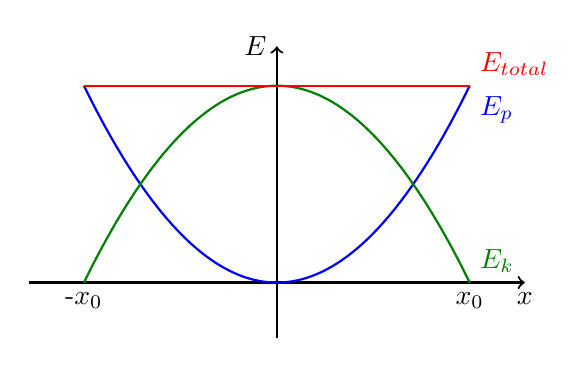
\begin{tikzpicture}[xscale=.7]
	\draw [thick, ->] (-4.5,0) -- (-3.5,0) node[below]{-$x_0$} -- (3.5,0) node[below]{$x_0$} -- (4.5,0) node[below]{$x$};
	\draw [thick, ->] (0,-0.7) --(0,3) node[left]{$E$};
	\draw [thick,color=blue,domain=-3.5:3.5,samples=40,smooth,variable=\x] plot (\x,{\x*\x*10/49}) node[below right]{$E_p$};
	\draw [thick,color=Green,domain=-3.5:3.5,samples=40,smooth,variable=\x] plot (\x,{2.5-\x*\x*10/49}) node[above right]{$E_k$};
	\draw [thick,color=red,domain=-3.5:3.5,samples=40,smooth,variable=\x] plot (\x,2.5) node[above right]{$E_\text{total}$};
	\end{tikzpicture}
	\end{minipage}
	\begin{minipage}{0.48\textwidth}
		\begin{center}
			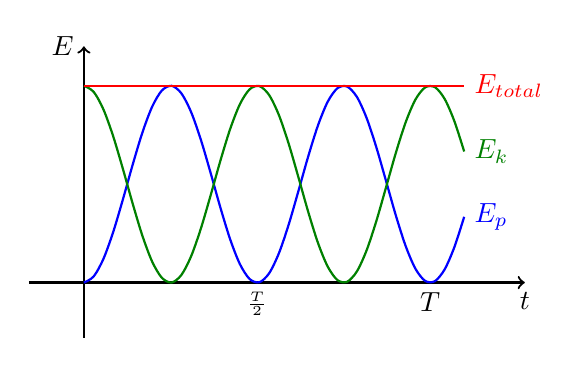
\begin{tikzpicture}[xscale=.7]
			\draw [thick, ->] (-1,0) --(8,0) node[below]{$t$};
			\draw [thick, ->] (0,-0.7) --(0,3) node[left]{$E$};
			\draw [thick,color=blue,domain=0:6.9,samples=40,smooth,variable=\x] plot (\x,{2.5*sin(\x r)*sin(\x r)}) node[right]{$E_p$};
			\draw [thick,color=Green,domain=0:6.9,samples=40,smooth,variable=\x] plot (\x,{2.5*cos(\x r)*cos(\x r)}) node[right]{$E_k$};
			\draw [thick,color=red,domain=0:6.9,samples=40,smooth,variable=\x] plot (\x,2.5) node[right]{$E_\text{total}$};
			\node[below] at (pi,0) {{\scriptsize $\frac{T}{2}$}};
			\node[below] at (2*pi,0) {$T$};
			\end{tikzpicture}
		\end{center}
	\end{minipage}

	
	vibrational energy of a mass-spring oscillator
\end{figure}

\example{A block of mass 150 g at the end of a spring oscillates with a period of 0.80 s. The maximum displacement from its rest position is 12 cm. Find the energy of the vibration.}

\solc\begin{equation*}
	E = \frac{1}{2}m\omega^2x_0^2 = \frac{1}{2}m\left(\frac{2\pi}{T}\right)^2x_0^2 = \frac{1}{2} \times 0.15 \times \frac{4\pi^2}{0.80^2}\times0.12^2 \approx 6.7\times10^{-2} \text{ J} \teoe
\end{equation*}

\question{An oscillator is given an energy of 20 mJ and starts to oscillate, it reaches an amplitude of 8.0 cm. If we want to double the amplitude, find the vibrational energy required.}

\subsection{damped oscillations}

total vibrational energy stays constant for an ideal system

but in reality, there are friction, resistance and viscous forces that oppose motion

\begin{ilight}
	amplitude of an oscillator decreases due to energy loss to friction, this is called \keypoint{damping}\index{damped oscillation}
\end{ilight} 

\subsubsection{light damping}

for a \keypoint{lightly-damped oscillator}\index{damped oscillation!light damping}, amplitude decreases \emph{gradually}

oscillator will not stop moving back and forth after quite a few oscillations

\begin{figure}[ht]
\centering
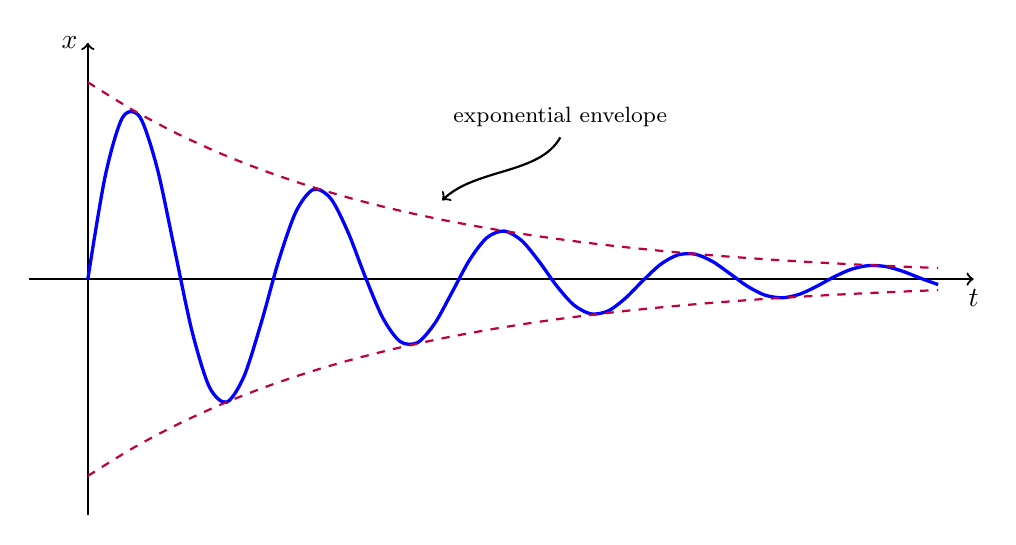
\begin{tikzpicture}[xscale=1.5]
\draw [thick, ->] (-0.5,0) --(7.5,0) node[below]{$t$};
\draw [thick, ->] (0,-3) --(0,3) node[left]{$x$};
\draw [very thick,color=blue,domain=0:7.2,samples=50,smooth,variable=\x] plot (\x,{2.5*sin(4*\x r)*exp(-\x/2.5)});
\draw [thick,color=purple,dashed,domain=0:7.2,samples=20,smooth,variable=\x] plot (\x,{2.5*exp(-\x/2.5)});
\draw [thick,color=purple,dashed,domain=0:7.2,samples=20,smooth,variable=\x] plot (\x,{-2.5*exp(-\x/2.5)});
\draw [thick,->] (4,1.8) node[above]{\footnotesize{exponential envelope}} to [out=-110, in=55] (3,1) ;
\end{tikzpicture}

\end{figure}

\cmt decrease in amplitude is \emph{non-linear} in time (exponential decay in many cases)

\cmt frequency and period are (almost) unchanged



\example{An oscillator is composed of a block of mass $m=250$ g and a spring of $k=1.6$ N/cm. It is displaced by 5.0 cm from its rest position and set free. (a) What is its angular frequency? (b) what is the initial vibrational energy? (c) After a few oscillations, 40\% of its energy is lost due to damping. What is its new amplitude?}

\sol angular frequency: $\omega = \sqrt{\frac{k}{m}} = \sqrt{\frac{160}{0.25}} \approx 25.3 \radps \,$

energy of oscillator: $E=\frac{1}{2}m\omega^2x_0^2 = \frac{1}{2} \times 0.25 \times 25.3^2 \times 0.050^2 = 0.20 \text{ J} $\footnote{An easier approach: $E = \frac{1}{2}kx_0^2 = \frac{1}{2} \times 160 \times 0.050^2 = 0.20 \text{ J}$.}

since $E \propto x_0^2$, so: $\frac{E'}{E} = \frac{x^{\prime2}_0}{x_0^2} \RA  60\% = \frac{x^{\prime2}_0}{x_0^2} \RA x'_0 = \sqrt{0.6} x_0 = \sqrt{0.6} \times 5.0 \approx 3.9$ cm \eoe

\question{A small toy boat of mass 360 g floats on surface of water. It is gently pushed down and then released. During the fist four complete cycles of its oscillation, its amplitude decreased from 5.0 cm to 2.0 cm in a time of 6.0 s. Find the energy loss.}

\subsubsection{heavy damping}

if resistive forces are too strong, there will be no oscillatory motion

the system will return to the equilibrium position very slowly

this system is said to be \keypoint{heavily damped}\index{damped oscillation!heavy damping}

\subsubsection{critical damping}

\keypoint{critical damping} is the border between light damping and heavy damping

it occurs when system returns to equilibrium in \emph{shortest} time without any oscillation\index{damped oscillation!critical damping}

\begin{figure}[ht]
	\centering
	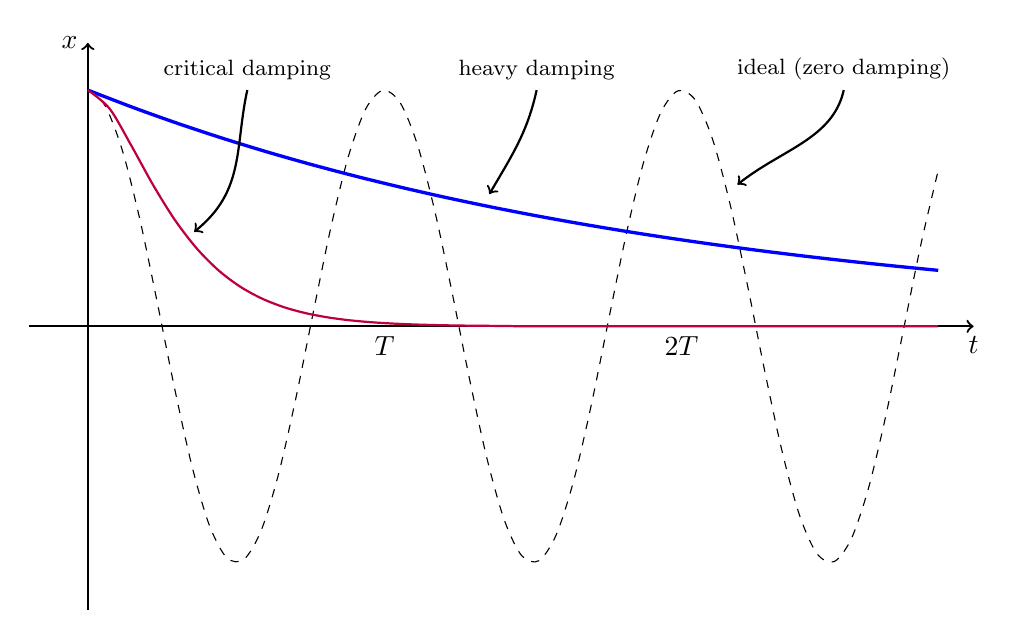
\begin{tikzpicture}[xscale=1.5,yscale=1.2]
	\draw [thick, ->] (-0.5,0) --(7.5,0) node[below]{$t$};
	\draw [thick, ->] (0,-3) --(0,3) node[left]{$x$};
	\draw [dashed,domain=0:7.2,samples=50,smooth,variable=\x] plot (\x,{2.5*cos(\x*2.5 r)});
	\draw [very thick,color=blue,domain=0:7.2,samples=20,smooth,variable=\x] plot (\x,{2.5*exp(-\x/5)});
	\draw [thick,color=purple,domain=0:7.2,samples=40,smooth,variable=\x] plot (\x,{2.5*(1+\x*2.5)*exp(-\x*2.5)});
	\draw [thick,->] (3.8,2.5) node[above]{\footnotesize{heavy damping}} to [out=-100, in=65] (3.4,1.4) ;
	\draw [thick,->] (1.35,2.5) node[above]{\footnotesize{critical damping}} to [out=-100, in=45] (0.9,1);
	\draw [thick,->] (6.4,2.5) node[above]{\footnotesize{ideal (zero damping)}} to [out=-100, in=45] (5.5,1.5) ;
	\draw (0.8*pi,0) node[below] {$T$};
	\draw (1.6*pi,0) node[below] {$2T$};
	\end{tikzpicture}
	
\end{figure}

\cmt critical damping is desirable in many engineering designs \footnote{When a damped oscillator is required, critically-damped system provides the quickest approach to equilibrium without overshooting, while lightly-damped system reaches the zero position quickly but continues to oscillate, and heavily-damped system reaches zero position in very long time.}

examples include door-closing mechanism, shock absorbers in vehicles and artillery, etc.



\subsection{forced oscillations}

\subsubsection{free \& forced oscillation}

an oscillator moving on its own with no gain or loss of energy is called \keypoint{free oscillation}

amplitude of the oscillation is constant, its frequency called \keypoint{natural frequency}

an oscillator may also move under an external driving force, it is \keypoint{forced oscillation}\index{forced oscillation}

frequency of forced oscillator tends to driving frequency after sufficiently long time

\subsubsection{resonance}

for a forced oscillation system, when frequency of driving force $f_\text{driving}$ is close to natural frequency $f_\text{natural}$, amplitude of oscillator increases rapidly

\begin{ilight}
	when driving frequency of external force equals natural frequency of the system, amplitude of the system becomes maximum, this phenomenon is called \keypoint{resonance}\index{resonance}
\end{ilight}


\begin{figure}[ht]
\centering
	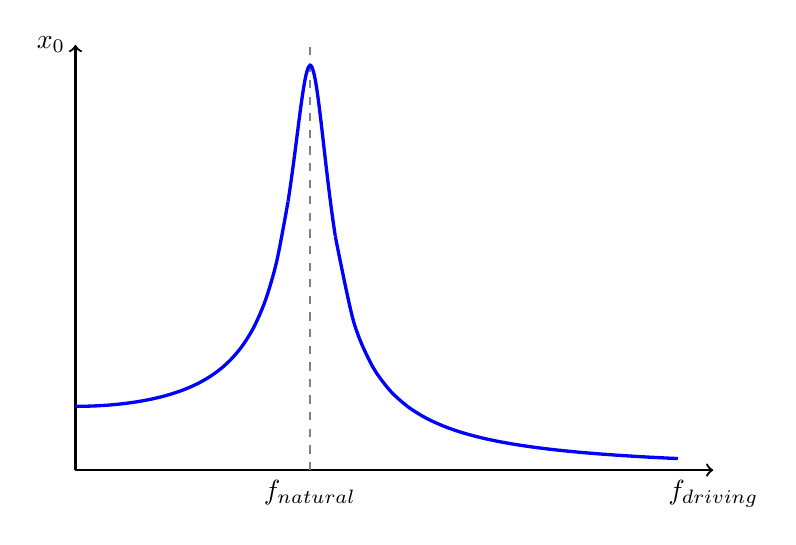
\begin{tikzpicture}[xscale=1.5,yscale=1.8]
	\draw [thick, ->] (0,0) -- (1.985,0) node[below]{$f_\text{natural}$} -- (5.4,0) node[below]{$f_\text{driving}$};
	\draw [thick, ->] (0,0) --(0,3) node[left]{$x_0$};
	\draw [thick,gray,dashed] (1.985,0) --++ (0,3);
	\draw [very thick,color=blue,domain=0:1.8,samples=20,smooth,variable=\x] plot (\x,{1.8/sqrt((4-\x*\x)*(4-\x*\x)+0.1*\x*\x)});
	\draw [very thick,color=blue,domain=1.8:2.2,samples=30,smooth,variable=\x] plot (\x,{1.8/sqrt((4-\x*\x)*(4-\x*\x)+0.1*\x*\x)});
	\draw [very thick,color=blue,domain=2.2:5.1,samples=20,smooth,variable=\x] plot (\x,{1.8/sqrt((4-\x*\x)*(4-\x*\x)+0.1*\x*\x)});
	\end{tikzpicture}
	
	resonance is achieved when $f_\text{driving} = f_\text{natural}$
	
	(amplitude tends to infinity if no damping)
\end{figure}


\cmt practical application of resonance

\begin{compactitem}
\item[-] microwave oven -- water molecules resonate at microwave frequency and vibrate greatly
\item[-] MRI (magnetic resonance imaging) --- precession of nuclei resonate at radio frequency, signals are processed to image nuclei of atoms inside a human body in detail
\item[-] radio/TV --- $RLC$ tuning circuits resonate at frequency of signals being received
\end{compactitem}

\cmt possible problems caused by resonance

\begin{compactitem}
\item[-] buildings during earthquake -- resonate at frequency of shockwaves and collapse
\item[-] car suspension system -- going over bumps may give large amplitude vibrations
\item[--] bridges and skyscrapers -- resonance due to wind conditions
\end{compactitem}

\subsubsection{damping \& resonance}

an oscillation system can be subject to both driving force and resistive force

resonance behaviour will be changed by damping effects

\cmt damping decreases amplitude of oscillation at all frequencies

greater damping causes resonance peak to become \emph{flatter}

engineering systems are often deliberately damped to minimise resonance effect

\cmt damping also shifts resonance frequency (slightly reduced for light damping)

\begin{figure}[ht]
	\centering
	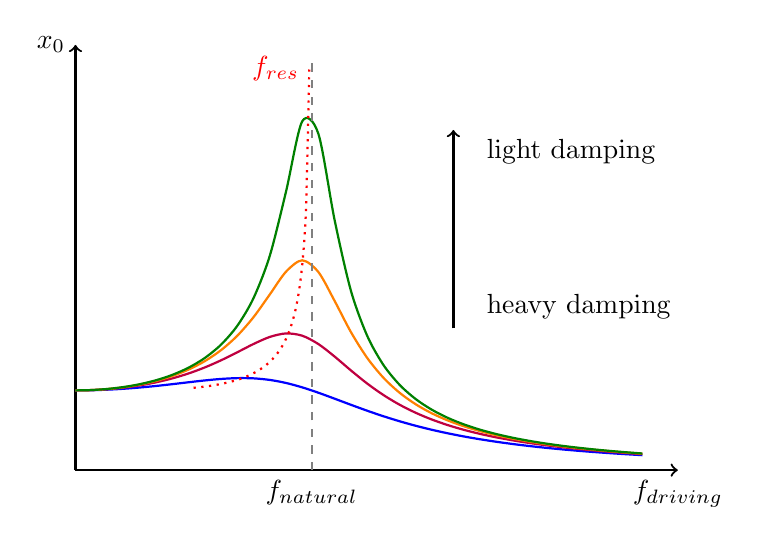
\begin{tikzpicture}[xscale=1.5,yscale=1.8]
	\draw [thick, ->] (0,0) -- (2,0) node[below]{$f_\text{natural}$} -- (5.1,0) node[below]{$f_\text{driving}$};
	\draw [thick, ->] (0,0) --(0,3) node[left]{$x_0$};
	\draw [thick,color=blue,domain=0:4.8,samples=36,smooth,variable=\x] plot (\x,{2.25/sqrt((4-\x*\x)*(4-\x*\x)+4*\x*\x)});
	\draw [thick,color=purple,domain=0:4.8,samples=36,smooth,variable=\x] plot (\x,{2.25/sqrt((4-\x*\x)*(4-\x*\x)+1.5*\x*\x)});
	\draw [thick,color=orange,domain=0:4.8,samples=36,smooth,variable=\x] plot (\x,{2.25/sqrt((4-\x*\x)*(4-\x*\x)+0.6*\x*\x)});
	\draw [thick,color=Green,domain=0:4.8,samples=36,smooth,variable=\x] plot (\x,{2.25/sqrt((4-\x*\x)*(4-\x*\x)+0.2*\x*\x)});
	\draw [thick,dotted,red,domain=1:1.98,samples=36,smooth,variable=\x] plot (\x,{9/16/sqrt(1-(\x*\x*\x*\x/16))}) node[left]{$f_\text{res}$};
	\draw  (3.4,1) node[above right]{heavy damping}  (3.4,2.4) node[below right]{light damping};
	\draw[thick,->] (3.2,1) -- (3.2,2.4);
	\draw [thick,gray,dashed] (2,0) -- (2,2.9);
	\end{tikzpicture}
	
	resonance effect for various damping conditions
\end{figure}

